\section{Design und Implementation}

\xxx

\subsection*{Mockups}

Als Diskussionsgrundlage und Vorlage für die Umsetzung wurden ca. 30 verschiedene \glspl{mockup} mit Balsamiq\footnote{\purl{https://balsamiq.com/products/mockups/}} umgesetzt.

\begin{figure}[H]
	\centering
	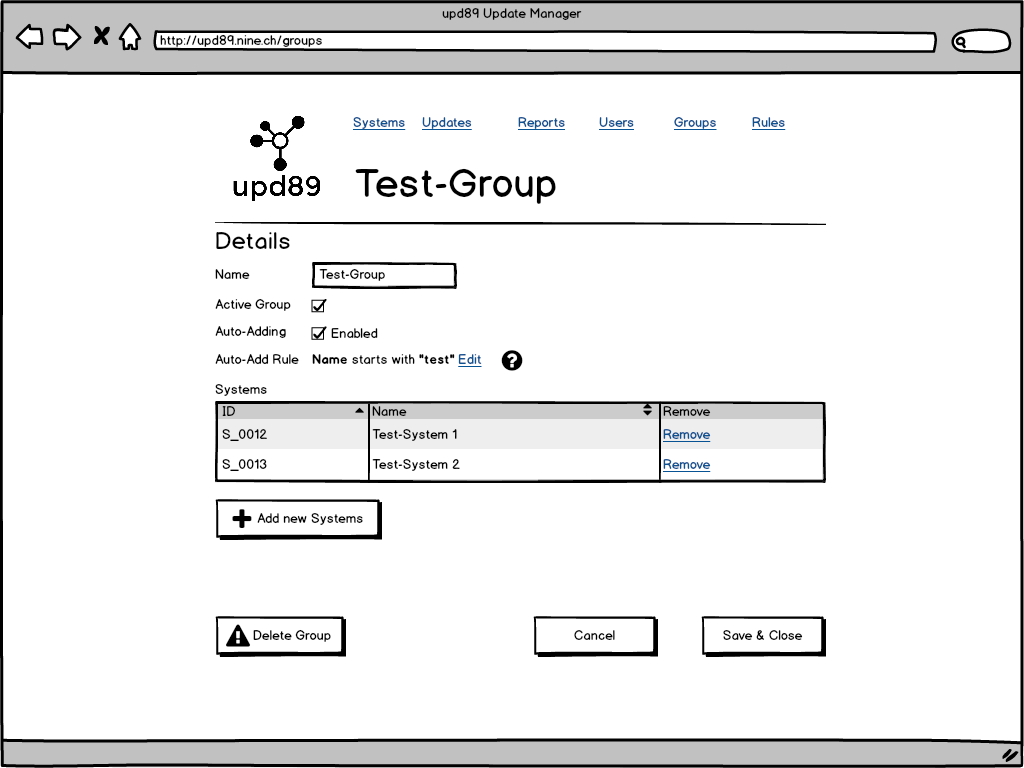
\includegraphics[width=\linewidth]{files/mockups/group_systems}
	\caption{Konzept Workflow-Feature}
	\label{fig:design:group_users_mockup}
\end{figure}

\begin{figure}[H]
	\centering
	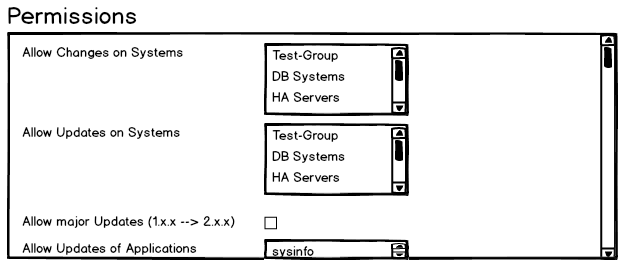
\includegraphics[width=\linewidth]{files/mockups/permission_1}
	\caption{Rechtesystem}
	\label{fig:design:permission_1}
\end{figure}

\begin{figure}[H]
	\centering
	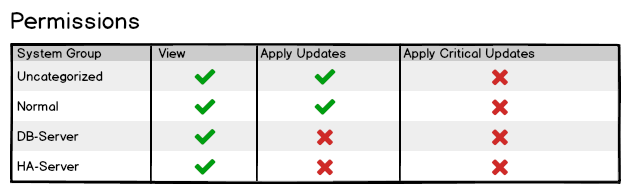
\includegraphics[width=\linewidth]{files/mockups/permission_2}
	\caption{Rechtesystem (Alternative)}
	\label{fig:design:permission_2}
\end{figure}

\begin{figure}[H]
	\centering
	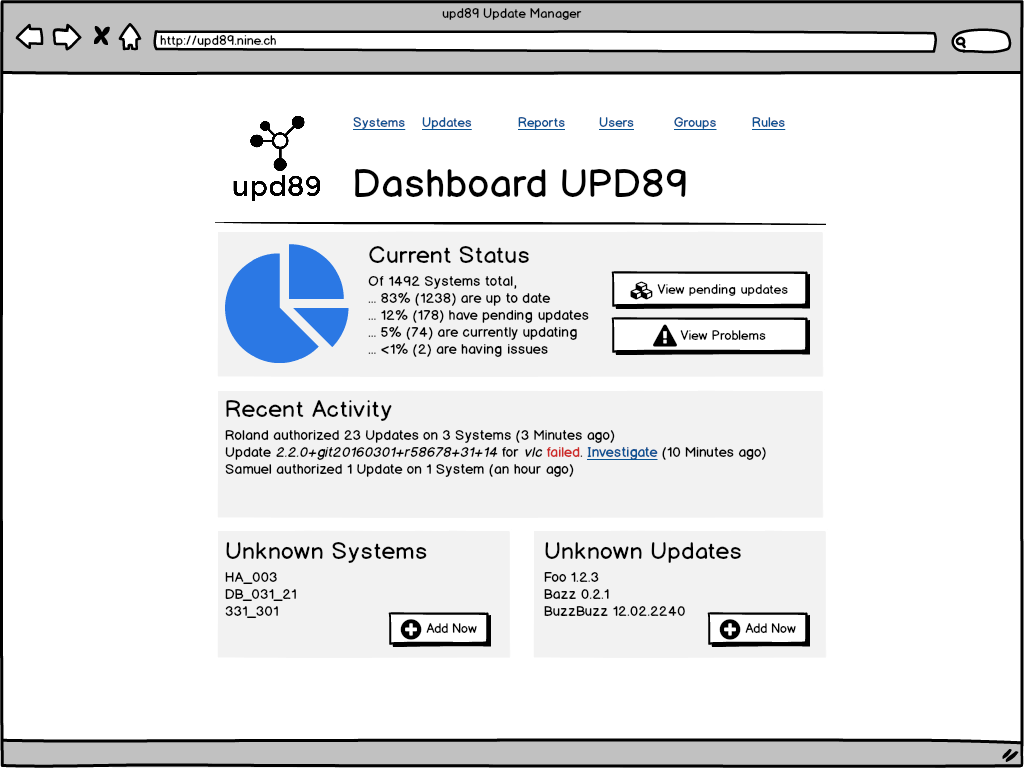
\includegraphics[width=\linewidth]{files/mockups/dashboard}
	\caption{Konzept des Dashboards}
	\label{fig:design:dashboard_mockup}
\end{figure}

\begin{figure}[H]
	\centering
	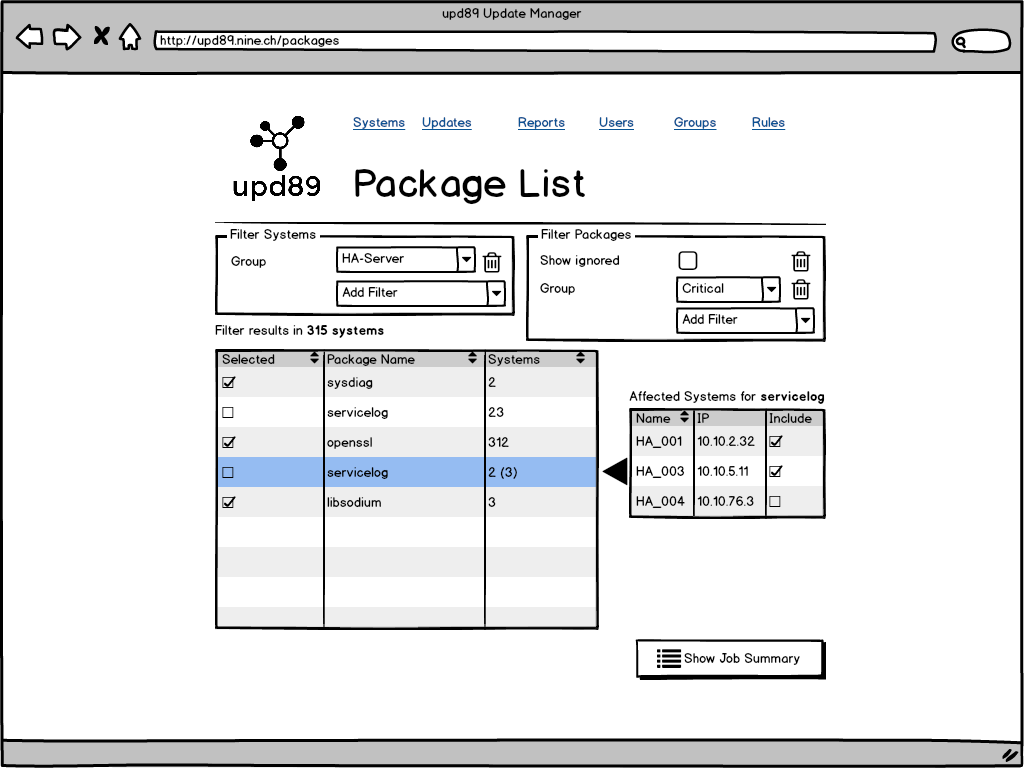
\includegraphics[width=\linewidth]{files/mockups/combo_view}
	\caption{Haupt-Ansicht mit Paket- und System-Filter}
	\label{fig:design:combo_view_mockup}
\end{figure}

\subsection*{User Interface}

Die Oberflächen halten sich mehrheitlich an die Mockups aus der Planung, einige Details wurden aber aufgrund von 

\begin{figure}[H]
	\centering
	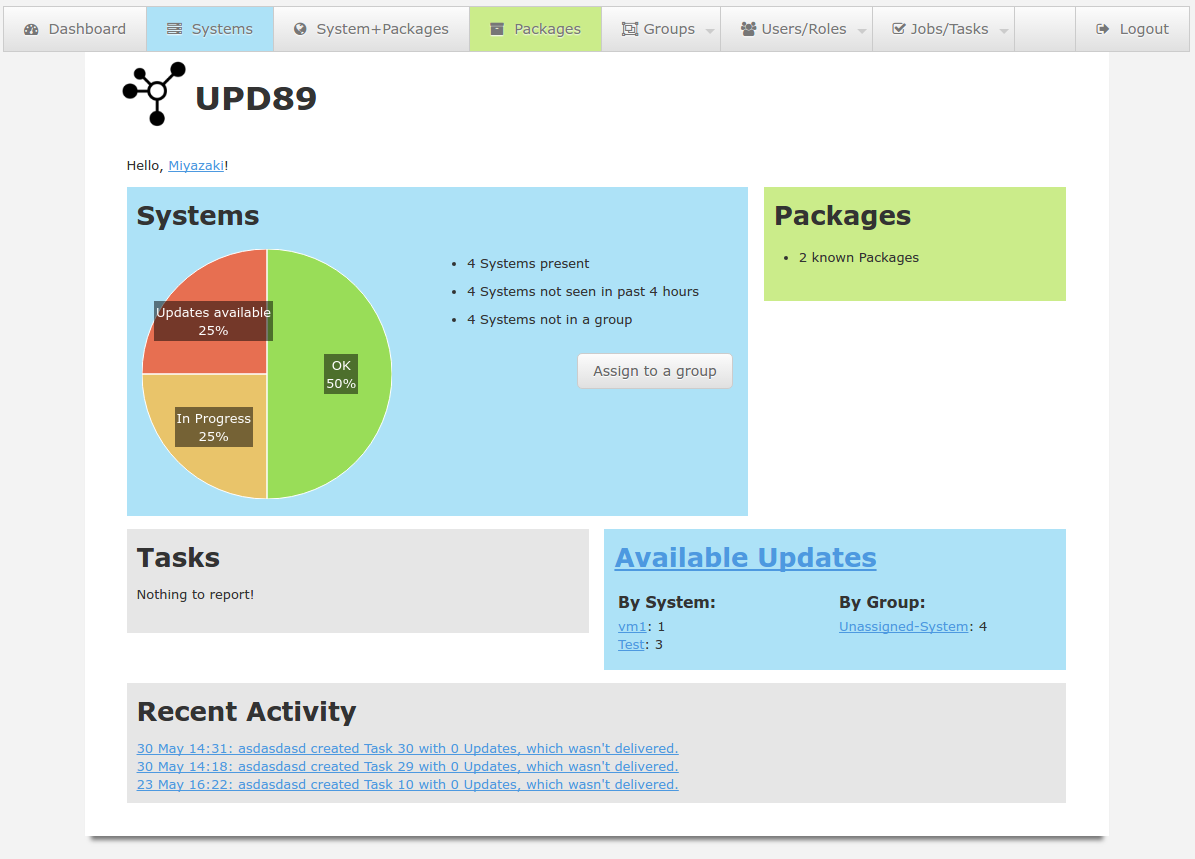
\includegraphics[width=\linewidth]{files/upd89-screenshot_dashboard}
	\caption{Umgesetztes Dashboard}
	\label{fig:design:dashboard}
\end{figure}

\subsubsection*{Farben}

Generell wurde das Interface eher schlicht gehalten. Grautöne sowie Rot, Gelb und Grün als Signalfarben lassen die Seiten übersichtlich und nicht überladen erscheinen.

\begin{figure}[H]
	\centering
	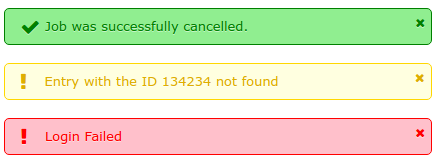
\includegraphics[width=0.5\linewidth]{files/messages}
	\caption{Beispiele der drei Hinweise 'Erfolg', 'Warnung', 'Error'}
	\label{fig:design:messages}
\end{figure}



\begin{figure}[H]
	\centering
	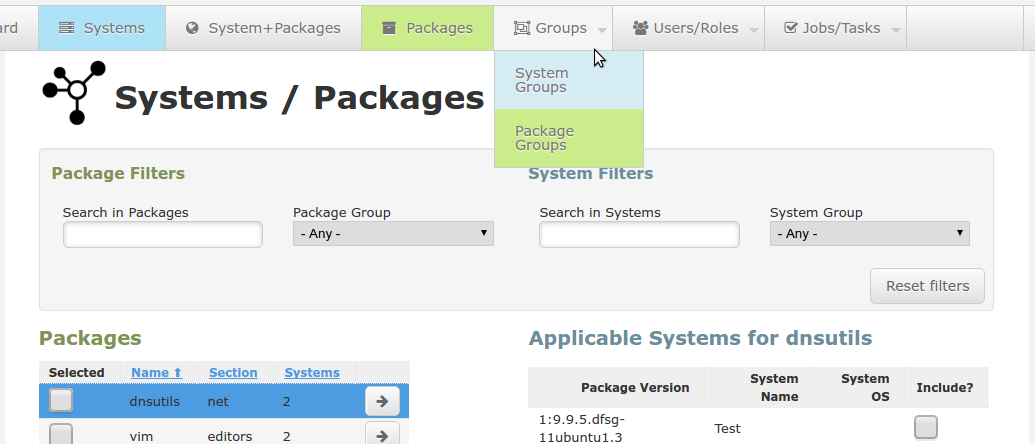
\includegraphics[width=\linewidth]{files/colors_pkg_sys}
	\caption{Simple Farb-Hinweise: Blau für Systeme, Grünlich für Pakete}
	\label{fig:design:color-code}
\end{figure}

\subsubsection*{Building Blocks}

Um verschiedene grafische Elemente konsistent gleich aussehen zu lassen, wurde das HTML Kickstart-Framework von Joshua Gatcke/99lime.com\footnote{\purl{http://www.99lime.com/elements/}} verwendet. Dadurch waren gewisse Funktionalitäten wie etwa das Menu oder die Hinweise bereits vorhanden.


Für die Icons wurde FontAwesome\footnote{\purl{http://fontawesome.io/}} verwendet.
